\documentclass[14pt]{article}

\usepackage[margin=1.5cm]{geometry}
\usepackage{enumerate}
\usepackage{amsmath,amssymb}
\usepackage{tikz}

\begin{document}

\begin{center}
Proficiency Exam 4 - Matrix Algebra
\end{center}

You will have 30 minutes to complete the exam.  You may use a calculator, but you must show all steps done to get full credit for completing the problem.  This means that if you use your calculator for anything other than arithmetic, you must indicate on your test paper what you did on the calculator.

\begin{enumerate}

\item Consider the network below.  How many paths of length 3 are there from node 1 to node 2?

\begin{center}
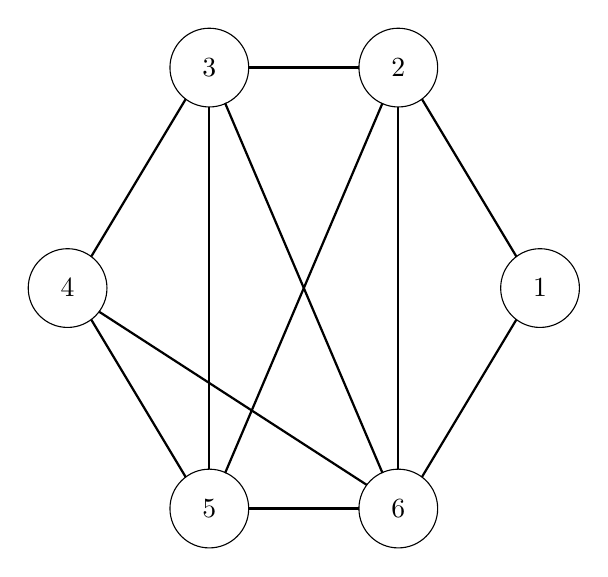
\begin{tikzpicture}
\node at (3,0) {1};
\draw (3,0) circle (0.5);
\node at (1.2,2.8) {2};
\draw (1.2,2.8) circle (0.5);
\node at (-1.2,2.8) {3};
\draw (-1.2,2.8) circle (0.5);
\node at (-3,0) {4};
\draw (-3,0) circle (0.5);
\node at (-1.2,-2.8) {5};
\draw (-1.2,-2.8) circle (0.5);
\node at (1.2,-2.8) {6};
\draw (1.2,-2.8) circle (0.5);

% node 1
\draw[thick] (2.7,0.4) -- (1.5,2.4); % 2
%\draw[thick] (2.6,0.3) -- (-0.8,2.5); % 3
%\draw[thick] (2.5,0) -- (-2.5,0); % 4
%\draw[thick] (2.6,-0.3) -- (-0.8,-2.5); % 5
\draw[thick] (2.7,-0.4) -- (1.5,-2.4); % 6

% node 2
\draw[thick] (0.7,2.8) -- (-0.7,2.8); % 3
%\draw[thick] (0.8,2.5) -- (-2.6,0.3); % 4
\draw[thick] (1,2.35) -- (-1,-2.35); % 5
\draw[thick] (1.2,2.3) -- (1.2,-2.3); % 6

% node 3
\draw[thick] (-1.5,2.4) -- (-2.7,0.4); % 4
\draw[thick] (-1.2,2.3) -- (-1.2,-2.3); % 5
\draw[thick] (-1,2.35) -- (1,-2.35); % 6

% node 4
\draw[thick] (-2.7,-0.4) -- (-1.5,-2.4); % 5
\draw[thick] (-2.6,-0.3) -- (0.8,-2.5); % 6

% node 5
\draw[thick] (0.7,-2.8) -- (-0.7,-2.8); % 6
\end{tikzpicture}
\end{center}

%\[
%\left[\begin{array}{ccccc}
%0 & 1 & 0 & 1 & 1 \\
%1 & 0 & 1 & 0 & 0 \\
%0 & 1 & 0 & 0 & 1 \\
%1 & 0 & 0 & 0 & 1 \\
%1 & 0 & 1 & 1 & 0
%\end{array}\right].
%\]
%How many paths are there of length 3 from node 3 to node 4?

\item Is the following linear function invertible?
\[
T(x,y,z) = \left[\begin{array}{c}1\\2\\3\end{array}\right](x-y) + \left[\begin{array}{c}1\\0\\-1\end{array}\right](x+y+2z)
\]

\item (TRUE or FALSE) Consider the statement and decide if it is true or false.  If true, provide reasoning.  If false, provide a counterexample.
\begin{center}
``Matrix multiplication is commutative; that is, $ AB = BA $ for square $ A $ and $ B $."
\end{center}

\item For what values of $ t $ is the matrix below invertible?
\[
\left[\begin{array}{cc}
t-1 & 3t-6 \\ t & -2t
\end{array}\right]
\]




























\end{enumerate}

\end{document}